%!TEX root = ../crux-sigconf.tex
\section{Budgeted Extraction}
\label{sec:problem}
We now define {\em budgeted crowd entity extraction} over structured domains and present an overview of our framework.
\subsection{Problem Definition}
\label{sec:extraction}
The problem of {\em crowdsourced entity extraction} seeks to extract entities that belong to $\domain$.  For large entity structured domains, one may need to issue a series of entity extraction queries at multiple nodes in  $\hierarchy$---often overlapping with each other---to ensure that the coverage across the domain is maximized. We refer to a series of  generalized $q^v(k,E)$ queries at different nodes $v \in \hierarchy$ as a {\em querying policy}.

Let $\pi$ denote a querying policy. A policy $\pi$ can select a query $q^v(k,E)$ multiple times. Let $C(\pi)$ denote the overall monetary cost of policy $\pi$. We define the gain of $\pi$, denoted by $\uentities(\pi)$, to be the total number of unique entities extracted when following $\pi$. There is a natural trade-off between the gain (i.e., the number of extracted entities) and the cost of policies. 

We require that the user will {\em only} provide a monetary budget $\tau_c$. The poset $\hierarchy$ and the possible query size and exclude list size configurations $(k,l)$ for each node are given as input by the application designer. Our goal is to identify the querying policy that maximizes the number of retrieved entities under the given budget constraint:

\begin{problem}[{\bf Budgeted Crowd Entity Extraction}]\label{prob:budgeted}
Let $\domain$ be an entity domain characterized by a poset $\hierarchy$. For each node $v \in \hierarchy$, let $K^v$ and $L^v$ be the sets of allowed query sizes and exclude list sizes for queries at node $v$. Let $\tau_c$ be a budget on the total cost of issued queries. Find a querying policy $\pi^*$ using queries $q^v(k,E)$ with $k \in K^v$ and $|E| = l \in L^v$ over nodes $v \in \hierarchy$ that maximizes $\uentities(\pi^*)$, the number of unique entities extracted, under the constraint $C(\pi^*) \leq \tau_c$.
\end{problem}
Note that the optimal policy not only specifies the nodes at which queries will be executed but also the size and exclude list of each query. The cost of a querying policy $\pi$ is $C(\pi) = \sum_{q \in \pi} c(q)$, where the cost of each query $q^v$ is defined according to a cost model specified by the user, is easy to compute. However, the number of unique entities extracted by a policy is not known upfront and needs to be estimated as we discuss in \Cref{sec:gainestimators}. Moreover, the problem of finding an optimal querying policy is NP-hard. 

\begin{theorem}[{\bf NP-Hardness}\label{thm:NPH}]
Problem~\ref{prob:budgeted} is NP-hard.
\end{theorem}
The proof is provided 
\iftr in \Cref{sec:prth1}
\fi
\ifpaper in our technical report~\cite{cruxsup} (with all other proofs)
\fi 
and is based on a reduction from the {\em unbounded knapsack} problem. This problem is a variation of the original 0-1 knapsack problem that places no upper bound on the number of copies of each kind of item. 

Finally, computing the total cost of a policy $\pi$ is easy. However, the gain $\uentities(\pi)$ of a policy $\pi$ is unknown as we do not know in advance the entities corresponding to each node in $\hierarchy$, and hence, needs to be estimated (see \Cref{sec:gainestimators}). 

\subsection{Query Response Model}
\label{sec:sampling}
To reason about the occurrence of entities as response to specific queries, we assume that each entity has an {\em unknown popularity value} with respect to crowd workers. Since workers are likely to return different answers based on how the query is phrased, this popularity can be different for different nodes in $\hierarchy$, and thus, is query-dependent. 
Given a query $q^v(1, \emptyset)$, the probability that we get entity $e$ in the result of $q^v$ is simply the popularity value of $e$ divided by the popularity value of all entities $e'$ that also satisfy the same predicate constraints. For example, if there are only two entities $e_1, e_2$ that satisfy the constraints of a query $q_1$, with popularity values $3$ and $2$, then the probability that we get $e_1$ on issuing a query $q_1(1, \emptyset)$ is 3/5. If an exclude list $E$ is specified, then the probability that we get $e \notin E$ is the popularity value of $e$ divided by the popularity values of all entities $e' \notin E$ also satisfying the predicates of $q^v$. 

Since workers are asked to provide a limited number of entities, each query can be viewed as taking a random sample from an unknown population of entities. We refer to the distribution characterizing the popularities of entities in a population as the {\em popularity distribution} of the population. We do not know the popularity distribution in advance; rather we use the samples retrieved by previous queries as a proxy to reason about this distribution. Also, it is not necessary that workers follow the same popularity distribution. Rather, the overall popularity distribution can be seen as an average of the popularity distributions across all workers. 
\iftr
Estimating average statistics across workers is standard practice in crowdsourcing applications~\cite{DasSarma:2016:TGO:2882903.2882953,trushkowsky:2013} since due to the sparsity in the number of answers per worker (especially since workers are fleeting on marketplaces), developing fine-grained models of worker responses can be challenging.
\fi

Estimating the gain of a query $q^v(k,E)$ at a node $v \in \hierarchy$ is equivalent to estimating the number of new entities extracted by taking additional samples from the population of $v$ given all the retrieved entities ({\em running sample}) associated with node $v$. Due to the structure of the poset we may retrieve entities for a node when issuing queries at other nodes. We discuss this form of {\em indirect sampling} in \Cref{sec:indirectsampling}. 

%\iftr
%\stitle{Popularities.} We assume that each underlying entity has a {\em fixed, unknown popularity value} with respect to crowd workers. Given a query $q(1, 0)$, asking for one entity and using an exclude list of size $0$, the probability that we will get entity $e$ that satisfies the constraints specified by $q$ is nothing but the popularity value of $e$ divided by the popularity value of all entities $e'$ that also satisfy the constraints in $q$. As an example, if there are only two entities $e_1, e_2$ that satisfy the constraints specified by a given query $q_1$, with popularity values $3$ and $2$,
%then the probability that we get $e_1$ on issuing a query $q_1(1, 0)$ is 3/5. 
%If an exclude list $S$ is specified, then the probability that we will get an entity $e \notin S$ is the popularity value of $e$ divided by the popularity values of all entities $e' \notin S$ also satisfying the constraints specified by $q$. Note that, we {\bf do not assume that all workers follow the same popularity distribution}. Rather the overall popularity distribution can be seen as an average of the popularity distributions across all workers.
%
%Thus, since workers are asked to provide a limited number of entities as response to a query, each entity extraction query can be viewed as taking a random sample from an unknown population of entities. In the rest of the paper, we will refer to the distribution characterizing the popularities of entities in a population of entities as the {\em popularity distribution} of the population. We note that this is equivalent to the underlying assumption in the species estimation literature~\cite{chao:1992} (\Cref{sec:gainestimators}).
%
%% We assume that the underlying entities exhibit different {\em popularity levels} with respect to crowd workers. These popularity levels can be formally defined using the notion of a probability distribution. In particular, the probability that an entity will appear as part of a query result depends on its {\em popularity} relative to the overall entity population. The popularity of an entity for a query $q$ is defined as the probability that this entity will appear in a query $q(1,0)$, i.e., a query asking for one entity from the population and using an exclude list of size zero. Since workers are asked to provide a limited number of entities as response to a query, each entity extraction query can be viewed as taking a random sample from an unknown population of entities. In the remainder of the paper, we will refer to the distribution characterizing the popularities of entities corresponding to a population as the {\em popularity distribution} of the population. 
%
%Then, estimating the gain of a query $q(k,l)$ at a node $v \in \hierarchy$ is equivalent to estimating the number of new entities extracted by taking additional samples from the population of $v$ given all the retrieved entities by past samples associated with node $v$~\cite{trushkowsky:2013}. 
%
%\stitle{Samples for a Node.} When extracting entities,  the retrieved entities for a node $v$ can correspond to two different kinds of samples: (i) those that were extracted by considering the {\bf entire population} corresponding to node $v$ (ii) and those that we obtained by sampling {\bf only a part of the population} corresponding to $v$. Samples for a node $v$ can be obtained either by querying node $v$ or by indirect information flowing to $v$ by queries at other nodes. We refer to the latter case as {\em dependencies across queries}. 
%\begin{figure}[h]
%	\begin{center}
%	\vspace{-10pt}
%	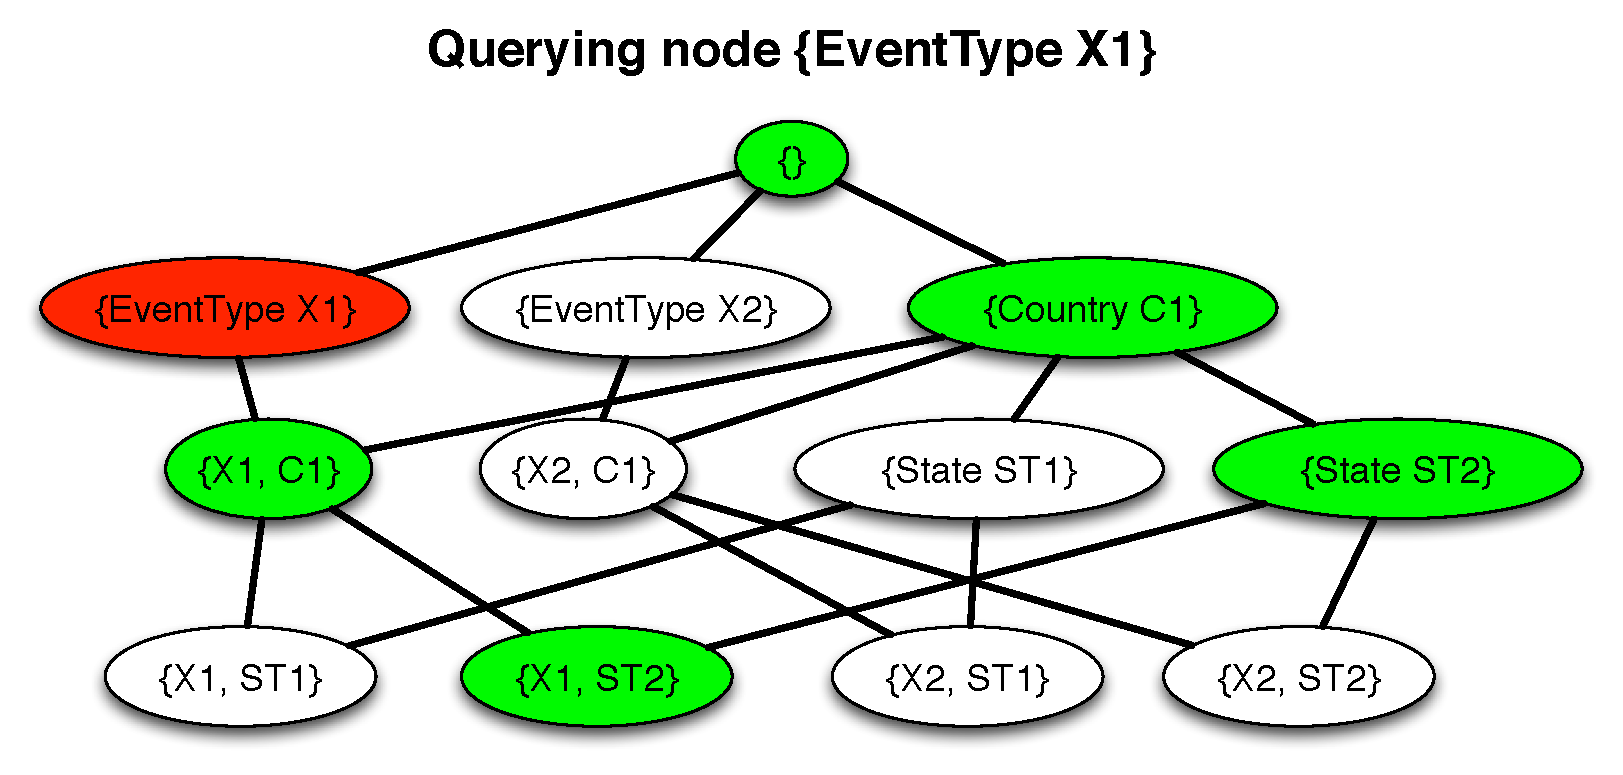
\includegraphics[clip,scale=0.3]{figs/exampleQuery.eps}
%	\caption{An example query that extract an entity sample from the red node. The nodes marked with green correspond to the nodes for which indirect entity samples are retrieved.}
%	\label{fig:query}
%	\vspace{-10pt}
%	\end{center}
%	\vspace{-5pt}
%\end{figure}
%
%We use an example considering the poset in \Cref{fig:eventslattice}, to illustrate these two cases. The example is shown in \Cref{fig:query}. Assume a query $q(k,0)$ issued against node \{EventType X1\}. Assume that the query result contains entities that correspond only to node \{X1,ST2\}. The green nodes in \Cref{fig:query} are nodes for which samples are obtained indirectly without querying them. Notice, that all these nodes are ancestors of \{X1,ST2\}. Analyzing the samples for the different nodes we have:
%\squishlist
%\item The samples corresponding to nodes \{X1, C1\} and \{X1,ST2\} were obtained by considering their {\em entire population}. The reason is that node \{EventType X1\} is an ancestor of both and the entity population corresponding to it fully contains the populations of both \{X1,C1\} and \{X1,ST1\}. 
%\item The samples corresponding to nodes \{ \}, \{Country C1\} and \{State ST2\} were obtained by considering only part of their population. The reason is that the population of node \{EventType X1\} does not fully contain the populations of these nodes. 
%\squishend
%
%Samples belonging to both types need to be considered when estimating the gain of a query at a node in $v \in \hierarchy$. To address this issue we merge the extracted entities for each node in $\hierarchy$ into a single sample and treat the unified sample as being extracted from the entire underlying population of the node. As we discuss later in \Cref{sec:solving} we develop querying strategies that traverse the poset $\hierarchy$ in a top-down approach, hence, the number of samples belonging in the first category, i.e., samples retrieved considering the entire population of a node, dominates the number of samples retrieved by considering only part of a node's population. Moreover, it has been shown by Hortal et al.~\cite{hortal2006evaluating} that several of the techniques that can be used to estimate the gain of a query (see \Cref{sec:gainestimators}) are insensitive to differences in the way the samples are aggregated.
%\fi
\subsection{CRUX Overview}
\label{sec:framework}
CRUX casts the budgeted crowd entity extraction problem as a multi-round adaptive optimization problem where at each round we solve the following subproblems: 
\squishlist 
\item \textbf{Estimating the Gain for a Query}~(\Cref{sec:gainestimators}). For each node $v \in \hierarchy$, consider the retrieved entities associated with $v$ and estimate the number of new unique entities that will be retrieved by a new query $q^v(k,E)$. The query gain is estimated for different query size and exclude list configurations.
\item \textbf{Detecting the Optimal Querying Policy}~(\Cref{sec:solving}). Using the gain estimates from the previous step, identify the query configuration $(k,l,v)$ that maximizes the total gain across all rounds given the budget constraint. When identifying the next query we do not explicitly optimize for the exclude list to be used. We rather optimize for the exclude list size $l$. Once the size is selected, the exclude list is constructed in a randomized fashion. We elaborate more on this in \Cref{sec:config}.
\squishend
CRUX iteratively solves the aforementioned problems until the entire budget is used. 
%\Cref{fig:framework} shows a high-level diagram of our proposed framework.
%
%\begin{figure}
%	\begin{center}
%	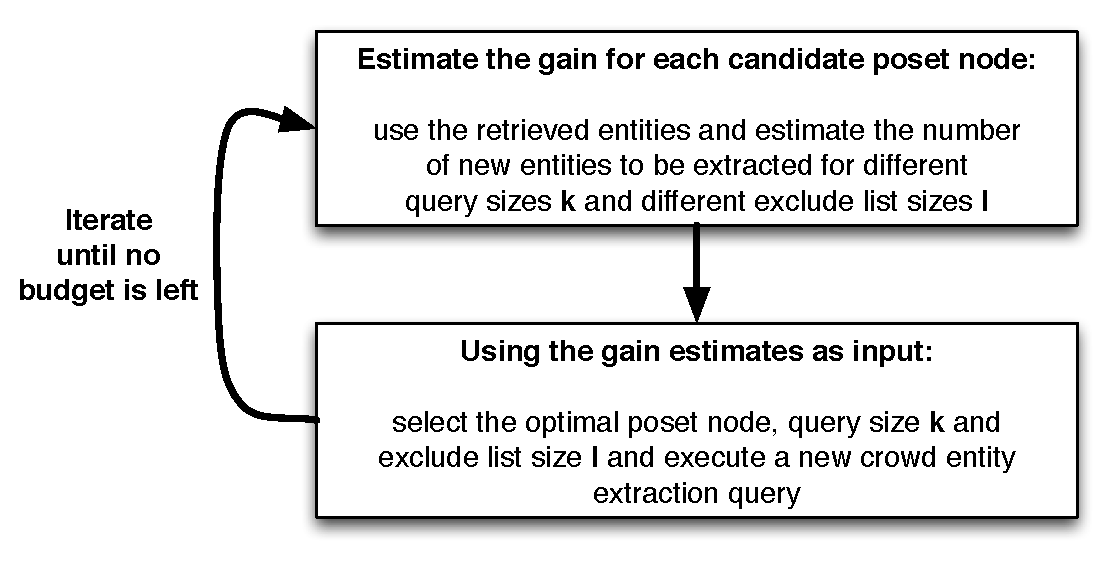
\includegraphics[clip,scale=0.43]{figs/framework.eps}
%	\caption{CRUX casts budgeted crowd entity extraction as a multi-round adaptive optimization problem. The main steps per round are shown.}
%	\label{fig:framework}
%	\vspace{-20pt}
%	\end{center}
%\end{figure}